\section{NXT Application Design}

\label{nxtdesign}

The application on the NXT brick should be responsible for aiming and firing the projectile at the target detected by the Kinect. This requires it to be able to convert the information it receives from the Kinect to usable data, predict where the target will be once positioning is done and position the cannon so that it hits the target when it fires. To ensure that the aiming is precise, a reset is required to have the cannon in the same position every time aiming is necessary. This process is illustrated below:

\begin{figure}[hbtp]
	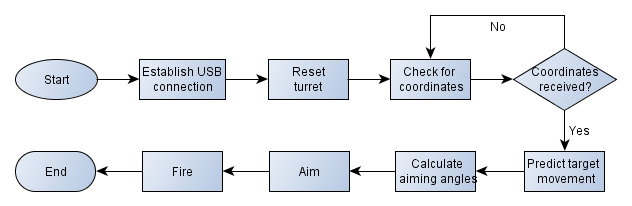
\includegraphics[scale=0.5]{img/nxtdesign.png}
	\caption{Process flow of NXT application}
	\label{nxtdesign}
\end{figure}

As shown, the flows is very linear: the application should first establish the USB connection to the Kinect via a computer, then reset position of the cannon and wait for the Kinect to supply coordinates. When the coordinates are received, the NXT should calculate where the target will be when the cannon is ready to fire, move the turret accordingly and fire.

This can be broken down into tasks for the NXT program, closely corresponding to the processes in \autoref{nxtdesign}:
\begin{itemize}
	\item Establish USB connection
	\item Reset turret position
	\item Poll for coordinates
	\item When coordinates are received, predict target movement and convert to degrees for the horizontal and vertical motors.
	\item Position horizontally
	\item Position vertically
	\item Fire cannon
\end{itemize}

It would be beneficial to have the same task establish connection to the Kinect and poll for coordinates, and have another task perform both the horizontal and vertical aim, for simplicity.

The conversion from Kinect coordinates to degrees for the motors should incorporate the mathematical equations from \autoref{maththeory} to compensate for gravity.

\subsection{Design Decisions}
First of all, the reset task should move the turret horizontally and vertically until the touch sensors receive input, and then move to the initial position. This will ensure that the aim is always precise and is a trivial task. The task should fire an event to the task handling interaction with the Kinect once the reset is complete, to start polling for a suitable target.

From the design of the USB protocol it is known that the data received will be two sets of (x,y,z)-coordinates which should be converted from USB-compatible char arrays to integers and stored in two 3D vectors, similar to how the image analyzer handles them, for consistency and ease of use. The task responsible for the USB connection should poll for coordinates every 1 ms, as mentioned in the NXTOSEK specifications \cite{osek_spec}. This should all be done in one task. Once coordinates are safely in place, the task should fire an event to let the aim-task know, that a target has been acquired.

Once coordinates are received and stored, the aim function should be able to predict from the vectors where the target will be once aim is complete, using velocity and a set deadline for when the aim should be completed. Afterwards the mathematical functions mentioned in \autoref{maththeory} should be applied, giving the amount of degrees each motor should move. The adjustment of motors can be concurrent or sequential, depending on the implementation. The task shall set an alarm with the deadline for aim done, and this alarm should start the fire task, which should then fire the projectile. The fire task is trivial, like the reset task.

